% arara: pdflatex
%        File: ComplexAnalysis.tex
%     Created: Sat Jun 24 03:00 PM 2023 B
% Last Change: Sat Jun 24 03:00 PM 2023 B
%
\documentclass[a4paper, 12pt]{article}
\usepackage[]{amsmath}
\usepackage{amsthm}
\usepackage{amssymb}
\usepackage{mathtools}
\usepackage{soul}
\usepackage[]{graphicx}
\graphicspath{ {./images/} }
\usepackage{caption}
\usepackage{subcaption}
\usepackage{hyperref}

\newtheorem{theorem}{Theorem}
\theoremstyle{definition}
\newtheorem{definition}{Definition}
\newtheorem{exercise}{Exercise}
\newtheorem{example}{Example}
\newtheorem{remark}{Remark}

\numberwithin{theorem}{section}
\numberwithin{definition}{section}
\numberwithin{exercise}{section}
\numberwithin{remark}{section}
\numberwithin{figure}{section}
\numberwithin{example}{section}

\newcommand{\R}{\mathbb{R}}
\newcommand{\C}{\mathbb{C}}
\newcommand{\intd}{\,\text{d}}

\renewcommand{\labelitemi}{$\circ$}
\renewcommand{\labelitemii}{*}

\DeclareMathOperator{\res}{Res}

\title{Complex Analysis Summary}
\author{Paul Joo-Hyun Kim}
\begin{document}
\maketitle
\tableofcontents
\setcounter{section}{-1}
\section{Preface}
This note is for people studying complex analysis,
and got lost in the middle with bunch of technical explanations.
I wil try my best to be succinct as possible,
stating important results (mostly without proof, but a bit of justification).

\textbf{Warning}: This summary note is not a substitute for the lecture note.
Make sure you study from lecture note!

\section{Complex Plane and M\"obius Maps}
\subsection{Complex Plane and Complex Infinity}
We will be working in what's known as the \textit{extended complex plane}.
Define the symbol $\C_{\infty} \coloneqq \C \cup \left\{ \underbrace{\infty}_{\text{Complex Infinity}} \right\}$;
that is, I refer to the space of complex numbers
and infinity.

Note that in $\C_{\infty}$, $\infty$ is different from infinity in real numbers.
$\infty \coloneqq \frac{1}{0}$ is a value that is not ``larger'' or ``smaller'' than any number
(since we are talking about complex number\dots), but rather
a number on a complex plane at a really far distance from origin.

It is \textbf{WRONG} to say:
\begin{itemize}
    \item $\infty \geq a$ for any $a \in \C_{\infty}$
    \item $\infty \leq a$ for any $a \in \C_{\infty}$
\end{itemize}
However, it is \textbf{CORRECT}\footnote{
    Subtlety here: it seems a bit dodgy to say $\infty = \infty$,
    but this is matter of definition;
    you won't really encounter this type of ``philosophical'' problem
    in your exam.
} to say:
\begin{itemize}
    \item $|\infty| \geq |a|$ for any $a \in \C_{\infty}$.
\end{itemize}
$\infty$ is not like a point on $\C$, but rather like a gigantic circle that you can never reach.

\subsection{M\"obius Maps}
\begin{definition}[M\"obius Map]
    $\psi : \C_{\infty} \rightarrow \C_{\infty}$ is a \textbf{M\"obius map} if:
    \begin{equation*}
        \psi \left( z \right) \coloneqq \frac{az + b}{cz + d}
    \end{equation*}
    where $
    \begin{pmatrix}
        a & b \\ c & d
    \end{pmatrix}
    $ is a nonsingular matrix.
    (This restriction removes the possibility of $\frac{0}{0}$,
    or trivial maps (eg: Constant function).)

    One needs to be careful when defining this function at infinity,
    but it should be sensible.\footnote{
    That said, if you are supposed to define what a M\"obius map is,
    you are \textbf{required} to definitions involving infinity as well.
    }
\end{definition}
\begin{exercise}[Composition of two M\"obius map is a M\"obius map]
    Show that for two M\"obius maps $\psi_1, \psi_2$,
    its composition $\psi_1 \circ \psi_2$ is also a M\"obius map.
\end{exercise}
\begin{remark}
    Consider the $2 \times 2$-matrix-to-M\"obius-map map as follows:
    \begin{equation*}
        f (A) \coloneqq
        \begin{pmatrix}
            a_{11} & a_{12} \\ a_{21} & a_{22}
        \end{pmatrix}
        \mapsto
        \frac{a_{11} z + a_{12}}{a_{21} z + a_{22}}
    \end{equation*}
    Then it turns out that
    $f\left( AB \right) = f(A) f(B)$
\end{remark}
\begin{exercise}[Decomposition of M\"obius maps]
    It turns out that M\"obius maps can be written as composition of
    \begin{itemize}
        \item translation
        \item dialation (``scaling by nonzero constant'')
        \item inversion ($z \mapsto \frac{1}{z}$)
    \end{itemize}
    Prove this. (Hint: You can do a constructive proof.)
\end{exercise}
M\"obius maps also has a very convenient property:
\begin{exercise}[Circline to Circline]
    Show that M\"obius maps map circlines to circline.
    (This means a line will either map to a circle or a line,
    and also a circle will either map to a circle or a line.)

    (Note: This is a boring long tedious proof, that probably won't be asked in exam,
    but don't take my word for it.)
\end{exercise}

\section{Complex Differentiability}
Complex differentiability is one of the highlights of the complex analysis.
\begin{definition}[Differentiable Function AKA Holomorphic Function]
    Take $a \in \C$.
    Let $f:U \rightarrow \C$ be a function where $U$ is a neighbourhood\footnote{Some open set containing $a$.} of $a$.
    Then $f$ is \textbf{(complex) differentiable} or \textbf{holomorphic} at $a$ if
    \begin{equation*}
        f'(a) = \lim_{z \rightarrow a} \frac{f(z) - f(a)}{z - a}
    \end{equation*}
    exists, and call it derivative of $f$ at $a$.
    If $f$ is differentiable for all points in $U$, then it is said to be
    differentiable/holomorphic on $U$.
\end{definition}
\begin{remark}
    Note that the definition seems to be have trivially extended from real analysis.
    \ul{However, there is a subtlety}.
    The limit does not approach just from positive or negative side,
    but from any direction. (Figure \ref{fig: Real and Complex Limit})
    \begin{figure}[tbp]
        \centering
        \begin{subfigure}[b]{0.5\textwidth}
            \centering
            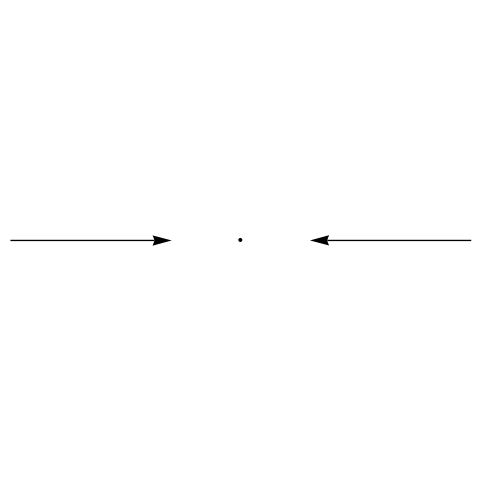
\includegraphics[width=\textwidth]{realLimit}
            \caption{Real Limit}
        \end{subfigure}
        \hfill
        \begin{subfigure}[b]{0.5\textwidth}
            \centering
            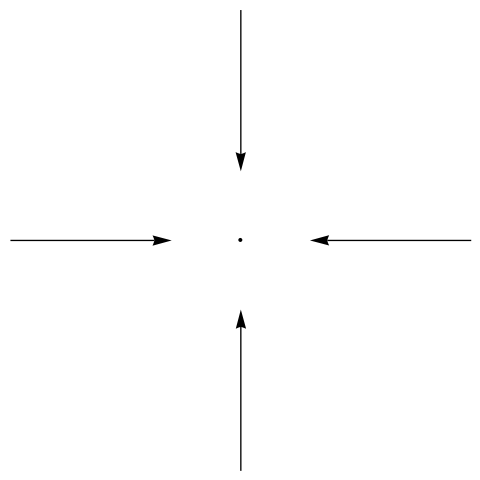
\includegraphics[width=\textwidth]{complexLimit}
            \caption{Complex Limit}
        \end{subfigure}
        \caption{Real limit (former) only concerns the approaching value from left and right side, but complex limit (latter) oncerns the approaching value from all direction.}
        \label{fig: Real and Complex Limit}
    \end{figure}
\end{remark}
\begin{exercise}[Differentiation Rules]
    Show that all differentiation rules from real analysis holds
    with holomorphic functions.
    \begin{itemize}
        \item Sum
        \item Product Rule
        \item Quotient Rule
        \item Chain Rule
    \end{itemize}
\end{exercise}
Due to the definition of complex limits being more restrictive,
a more nontrivial result follows.
\begin{exercise}[Cauchy-Riemann Equations]
    Let $a \in \C$ and $U$ be a neighbourhood of $a$.
    $f : U \rightarrow \C$ be holomorphic $a$.
    Write $f(z) = u(x,y) + i v(x,y)$ where $u,v$ are real functions
    and $z = x + iy$ where $x,y \in \R$.
    Then $\partial_x u, \partial_y u, \partial_x v, \partial_y v$ all exist,
    and the following \textbf{Cauchy-Riemann equations} hold:
    \begin{align*}
        \partial_x u &= \partial_y v \\
        \partial_x v &= - \partial_y u
    \end{align*}
(Hint: Figure \ref{fig: Real and Complex Limit} might give you an insight.)
\end{exercise}
\begin{remark}
    If Cauchy-Riemann does not hold, then it must mean that $f$ is not holomorphic! (Consider $f(z) = \bar{z}$. Cauchy-Riemann does not hold for any point, so it is nowhere holomorphic.)
\end{remark}
\begin{exercise}
    If $f(z) = u(x,y) + i v(x,y)$ is holomorphic on $U$,
    and $u,v$ are twice differentiable,
    deduce that $u$ and $v$ are \textit{harmonic}, that is,
    they satisfy the Laplace equation $\Delta u = \Delta v = 0$.
\end{exercise}
\begin{remark}
    It turns out complex plane reveals a lot about solving Laplace equation!
\end{remark}
Here is another kicker:
\begin{exercise}[Cauchy-Riemann to Holomorphic]
    If the partial derivatives exist and are continuously differentiable,
    Cauchy-Riemann implies holomorphicity.
\end{exercise}
\begin{remark}
    This means if you check that Cauchy-Riemann holds, you can immediately assume you can construct an analytic function!
\end{remark}
Holomorphic functions also have Taylor expansion:
\begin{remark}[Holomorphic functions have Taylor expansion]
    If $f$ is holormorphic at $a$, then
    in a neighbourhood of $a$, you can write
    \begin{equation*}
        f(z) = \sum_{n=0}^{\infty} c_n \left( z-a \right)^n
    \end{equation*}
    All the formulae for Taylor expansion holds (term-by-term differentiation, etc.)
\end{remark}
\begin{example}[Common Function Definitions]
    Here are definitions for some of the functions.
    \begin{align*}
        e^z = \exp z &\coloneqq \sum_{n=0}^{\infty} \frac{z^n}{n!} \\
        \cos{z} &\coloneqq \sum_{n=0}^{\infty} \left( -1 \right)^n \frac{z^{2n}}{\left( 2n \right)!} \\
        \cos{z} &\coloneqq \sum_{n=0}^{\infty} \left( -1 \right)^n \frac{z^{2n+1}}{\left( 2n + 1\right)!}
    \end{align*}
\end{example}
\begin{exercise}
    Show that
    \begin{align*}
        \cos{z} &= \frac{e^{iz} + e^{-iz}}{2} \\
        \sin{z} &= \frac{e^{iz} - e^{-iz}}{2i}
    \end{align*}
\end{exercise}
\begin{exercise}
    Show that $\exp \left( z+w \right) = \exp (z) \exp (w)$
\end{exercise}
\section{Branch Cut}
Sometimes, there is just no sensible way to define a function that it is holomorphic everywhere\dots
Two of the unfortunate (or fortunate) functions is the logarithm and square root.
We will first introduce the logarithm function.

Define logarithm function as:
\begin{equation*}
    \log z \coloneqq \log |z| + i \theta
\end{equation*}
where $\theta$ is the argument of $z$.

\begin{exercise}
    Verify that $\exp \left( \log z \right) = z$.
\end{exercise}

The choice of the interval for $\theta$ changes the behaviour of $\log z$ function.
For example, one could take the interval to be $\left[ 0, 2\pi \right)$,
or one could take it to be $\left[ - \pi, \pi \right)$,
or even just $\left[a, a + 2\pi\right)$ for some $a \in \R$.

The problem is that for given $z$, the argument of $z$ is not unique,
and if you try to define it continuously around a circle,
you will find that it is not possible\dots
(Figure \ref{fig: arg z multivalued}).
This means there needs to be some sort of contour from 0 that the function is not continuous on.
This is known as a \textbf{branch cut}, and you have total freedom to choose
based on what problem you want to solve.

\begin{figure}[tbp]
    \centering
    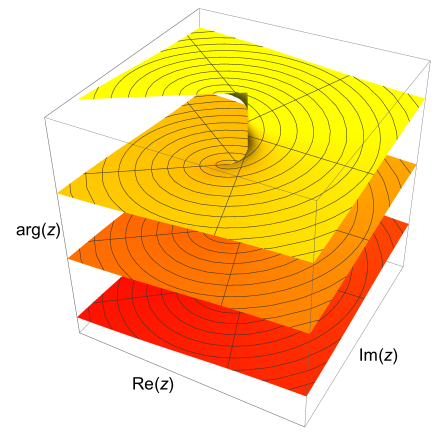
\includegraphics[scale=0.5]{argz}
    \caption{$\arg z$ being multivalued results in the need to introduce branch cut for logarithm.}
    \label{fig: arg z multivalued}
\end{figure}

\begin{example}[Where do we use branch cut?]
If you want to solve a problem with a fracture in an elastic solid (Figure \ref{fig: Crack Tip}),
one standard way to solve it is to find some holomorphic function outside of the crack $\left[ -c,c \right]$
satisfying some condition.
\begin{figure}[tbp]
    \centering
    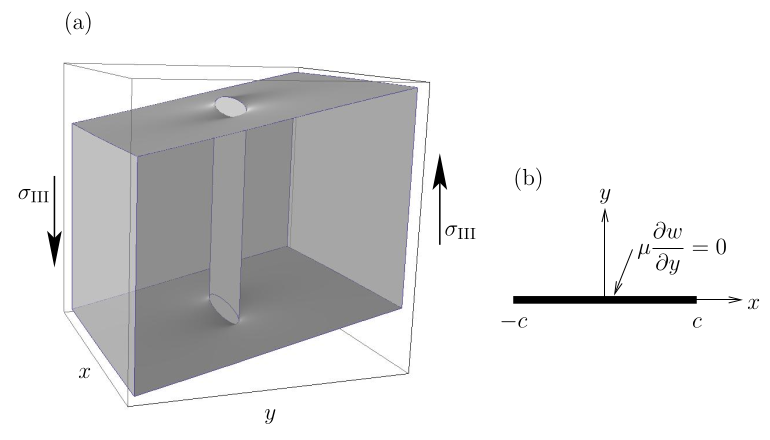
\includegraphics[scale=.5]{crackTip}
    \caption{Fracture in elastic material.}
    \label{fig: Crack Tip}
\end{figure}
It turns out that there is no function that is holomorphic everywhere satisfying that,
so you would define a ``branch cut'' to be the straight line $\left[ -c,c \right]$ to resolve it.
Then it is possible to define a function that is continuous away from the crack.
\end{example}

\begin{remark}
    When I say I am defining a branch cut,
    it means I am defining the function to be continuous away from the branch cut.
    \textbf{I am not the value of the function} at the function.
\end{remark}

Branch cuts are something that honestly makes more sense once you \textbf{played around with it for a while}.

\begin{example}[Logarithm: branch cut along positive real axis]
    See Figure \ref{fig: Log Positive Real} for the diagram of a branch cut along positive real axis.
    $\log z \coloneqq \log |z| + \theta i$ where $\theta \in \left[ 0, 2\pi \right)$ has a branch cut along positive real axis.
    Right above the positive real axis, $\theta$ takes the value 0, so $\left(\log x\right)_{+} = \log |x|$.
    On the other hand, right below the positive real axis, $\theta$ takes the value $2\pi$, so $\left( \log x \right)_{-} = \log |x| + 2\pi i$

    So you might ask: \textit{What is $\log z$ where $z \in \R^{>0}$?} and the answer is,
    you are asking the wrong question, because we can only define the ``limiting value'' on each side of the branch cut,
    NOT on the branch cut.
    \begin{figure}[tbp]
        \centering
        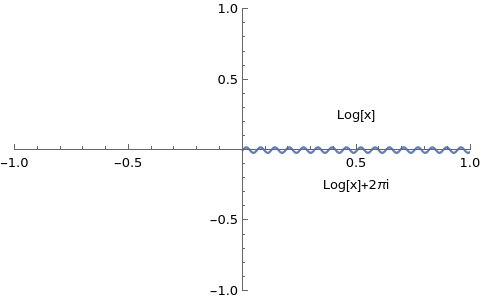
\includegraphics{logpositivereal}
        \caption{Logarithm function with branch cut along the positive real axis}
        \label{fig: Log Positive Real}
    \end{figure}
\end{example}
\begin{example}[Logarithm: branch cut along positive real axis]
    This time take $\theta \in \left[ -\pi, \pi \right)$.
    On the right side of the branch cut, we have $\theta = \pi$, so
    $\left( \log \left( yi \right) \right)_{+} = \log{y} + \pi i$,
    whereas on the left side, we have $\theta = -\pi$, so
    $\left( \log \left( yi \right) \right)_{-} = \log{y} - \pi$.

    \begin{figure}[tbp]
        \centering
        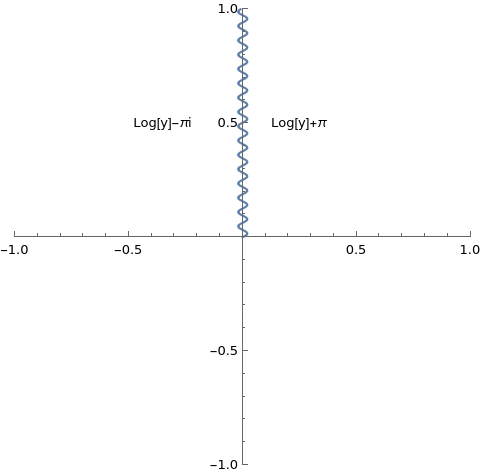
\includegraphics{logpositiveimaginary}
        \caption{Logarithm function with branch cut along the positive imaginary axis \textbf{Edit:} $\pi$ on the right side should be $\pi i$}
        \label{fig: Log Positive Imaginary}
    \end{figure}
\end{example}

\begin{exercise}[Square Root]
    Consider the definition of square root as given:
    \begin{equation*}
        z^{1/2} \coloneqq |z|^{1/2} e^{i \theta / 2}
    \end{equation*}
    (Note that I've just taken ``half'' as exponent in the polar form.)

    Define the branch cut along the negative real axis and evaluate $i^{1/2}$ in this branch.
    Define the branch cut along the negative imaginary axis and evaluate it again.
\end{exercise}
\begin{remark}
    In both square roots and logarithms, there was a point which the branch cut naturally starts from.
    These points are called \textbf{branch point};
    these are the points that you cannot avoid having a branch cut.
\end{remark}
\begin{remark}
    There is absolutely no need for a branch cut to be a straight line,
    and in some cases, it is more natural to define the branch cut in some other way (out of scope, however)
    Figure \ref{fig: spiral} is a classic example of non-straight branch.
    \begin{figure}[tbp]
        \centering
        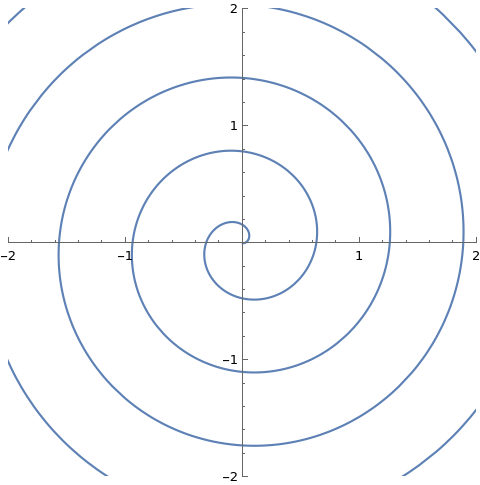
\includegraphics[scale=0.6]{spiral}
        \caption{A possible branch from a branch point (taken to be origin); a bit more complicated to describe, and often times, drawing this diagram might just be sufficient.}
        \label{fig: spiral}
    \end{figure}
\end{remark}
\begin{exercise}
    Try defining some branch cuts of $\left( 1+z \right)^{1/2}$.
    What is the branch point in this case?
\end{exercise}
\begin{example}[Square Root Branch Cut of Elastic Crack]
    \label{eg: Square Root Branch Cut of Elastic Crack}
    Suppose you want to define the branch of the function $\left( z^2 - 1 \right)^{1/2}$
    such that it is holomorphic away from the branch cut $\left[ -1,1 \right]$.

    Consider writing the function in a following way:
    \begin{equation*}
        \left( z^2 - 1 \right)^{1/2} = \left( z-1 \right)^{1/2} \left( z+1 \right)^{1/2}
    \end{equation*}
    Now note that $\left( z-1 \right)^{1/2}$ and $\left( z+1 \right)^{1/2}$ need branch cuts.
    One way to define them is through:
    \begin{align*}
        \left( z-1 \right)^{1/2} &= r_1^{1/2} e^{i\theta_1 / 2} \\
        \left( z+1 \right)^{1/2} &= r_2^{1/2} e^{i\theta_2 / 2}
    \end{align*}
    where $\theta_1, \theta_2 \in \left[ -\pi, \pi \right)$ (See Figure \ref{fig: Crack Tip 2}\footnote{
            The angle range is not a mistake, even though it might seem a bit unintuitive.
    })
    \begin{figure}[tbp]
        \centering
        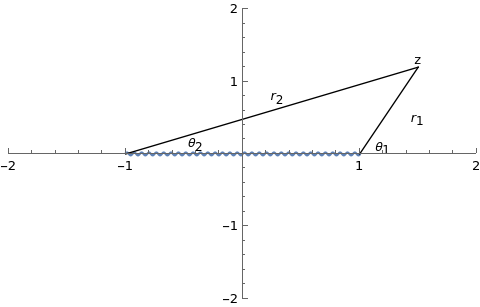
\includegraphics{crackTip2}
        \caption{$r_1, r_2, \theta_1, \theta_2$ as shown. The point on the upper right is the $z$. Branch cut is at $[-1,1]$.}
        \label{fig: Crack Tip 2}
    \end{figure}
    Hence, we get our branch cut between -1 and 1:
    \begin{equation*}
        \left( z^2 - 1 \right)^{1/2} = r_1^{1/2} r_2^{1/2} e^{i \left( \frac{\theta_1 + \theta_2}{2} \right)}
    \end{equation*}
\end{example}
\begin{exercise}
    Show that the branch cut defined on Example \ref{eg: Square Root Branch Cut of Elastic Crack}
    has different limiting values across the branch cut.
    \textbf{Again, the angle range given is not a mistake!}
\end{exercise}
\begin{exercise}
    Suppose the angle ranges are given to be $\theta_1 \in \left[ 0, 2\pi \right)$, $\theta_2 \in \left[ -\pi, \pi \right)$.
    Verify that the branch cuts are $(-\infty, -1] \cup [1, \infty) \subset \R$;
    that is, $\left( z^2 - 1 \right)^{1/2}$ has jump discontinuity across
    those intervals.

    (Hint: Sketch of the branch cut diagram is given as Figure \ref{fig: Crack Tip Out})
    \begin{figure}[tbp]
        \centering
        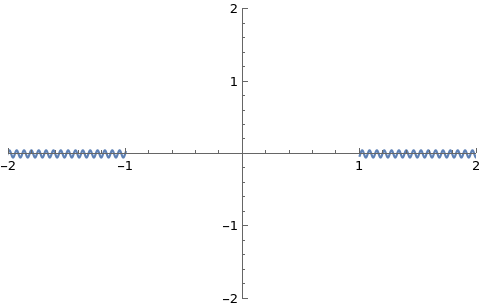
\includegraphics[scale=0.7]{crackTipOut}
        \caption{Branch cut diagram for $\theta_1 \in \left[ 0, 2\pi \right)$ and $\theta_2 \in \left[ -\pi, \pi \right)$}
        \label{fig: Crack Tip Out}
    \end{figure}
\end{exercise}
\begin{exercise}
    Let $f(z) = \left( k-i \right)^{1/2}$ with the branch cut at $i \left[ 1, \infty \right)$ (positive imaginary axis starting from $i$, the branch point).
    Show that $f(0) = e^{-i \pi/4}$.
\end{exercise}


\section{Paths and Integration}
You may have seen paths (AKA curves or lines) and integral along them
in multivariable calculus.
The complex analysis version is similar, but from a different perspective.
\subsection{Paths}
\begin{definition}[Path]
    Let $a < b$.
    $\gamma:[a,b] \rightarrow \C$ is a \textbf{path} if it is a continuous function.
    It is \textbf{closed} if $\gamma(a) = \gamma(b)$, that is, if the endpoints coincide.
\end{definition}
Tangent vector of a curve was an important concept in curves in MVC.
Similarly, one could define the notion of it in complex analysis by
introducing the ``derivative''.
\begin{definition}[Differentiability of Path]
    Path $\gamma:\left[ a,b \right] \rightarrow \C$ is \textbf{differentiable} at $t_0$ if
    its real and imaginary parts are differentiable at $t_0$,
    which is equivalent to saying
    \begin{equation*}
        \lim_{t \rightarrow t_0} \frac{\gamma(t) - \gamma(t_0)}{t-t_0}
    \end{equation*}
    exists.
    If so, we write this limit as $\gamma'(t_0)$.

    If $\gamma'(t)$ is continuous, then we say the path is in $C^1$.
\end{definition}
\begin{exercise}[``Tangent'']
    Show that $\gamma'(t)$ (if it exists) characterizes the tangent direction of the path $\gamma$.
    (Hint: Turn it into an MVC problem!)
    Explain what happens at $t_0$ if $\gamma'(t_0) = 0$.
\end{exercise}
\begin{example}
    \begin{figure}[tbp]
        \centering
        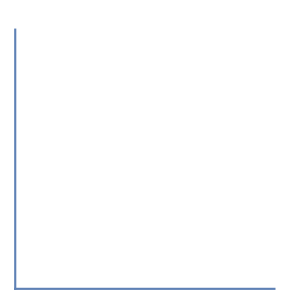
\includegraphics{pathRightAngle}
        \caption{Path given by piecewise $C^1$ path.}
        \label{fig: Path Right Angle}
    \end{figure}
    Consider
    \begin{equation*}
        \gamma(t) \coloneqq
        \begin{cases}
            t^2 &-1 \leq t \leq 0 \\
            it^2& 0 \leq t \leq 1
        \end{cases}
    \end{equation*}
    This is a piecewise $C^1$ path. See Figure \ref{fig: Path Right Angle}
    Note that $\gamma'(0) = 0$, so there is no ``tangent'' at the sharp corner.
\end{example}
\begin{example}[Circle]
    \textbf{One of the most important paths!}
    You can parameterize a circle with center $z_0$ and radius $r$ by:
    \begin{equation*}
        \gamma(t) = z_0 + r e^{it}
    \end{equation*}
    where $t \in \left[ 0, 2\pi \right]$.
    (You could also do $\gamma(t) = z_0 + r e^{2\pi i t}$ where $t \in \left[ 0, 1 \right]$)
    
    Note that the direction is counterclockwise.
\end{example}

\subsection{Complex Path Integral}
\begin{definition}[Complex Integral]
Given a complex function $F(t) = x (t) + i y(t)$,
one could define the integral over $t\in \left[ a,b \right]$ to be
\begin{equation*}
    \int_{a}^b F(t) \intd t \coloneqq \int_a^b x(t) \intd t + i \int_a^b y(t) \intd t
\end{equation*}
\end{definition}
\begin{exercise}
    Prove that, just like in real analysis, you can bound by the integral of the modulus of integrand; that is:
    \begin{equation*}
        \left| \int_a^b F(t) \intd t \right| \leq \int_a^b \left| F(t) \right| \intd t
    \end{equation*}
\end{exercise}
\begin{definition}[Path Integral]
    Given piecewise $C^1$ path $\gamma:[a,b] \rightarrow \C$ and $f: \C \rightarrow \C$, then
    \begin{equation*}
        \int_{\gamma} f(z) \intd z \coloneqq \int_{a}^b f\left( \gamma(t) \right) \gamma'(t) \intd t
    \end{equation*}
\end{definition}
\begin{remark}
    For remembering the definition,
    you can treat it as substitution rule in real integral:
    \begin{align*}
        z &= \gamma(t) \\
        \intd z &= \gamma'(t) \intd t
    \end{align*}
\end{remark}
\begin{example}[Terms in Taylor Around a Circle\footnote{Come back to this after you do residue theorem as well!}]
    \label{eg: Taylor Term Circle Integral}
    Given unit circle around origin (counterclockwise) as the path,
    let's compute the path integral of $f(z) = z^n$ where $n \in \mathbb{Z}$.
    \begin{align*}
        \int_{\gamma} z^n \intd z &= 
        \int_{0}^{2\pi} \left( e^{it} \right)^n e^{it}i \intd t \\
        &= \int_{0}^{2\pi} e^{it\left( n+1 \right)}i \intd t \\
        &= 
        \begin{cases}
            \frac{1}{n+1} \left[ e^{it(n+1)}i \right]_{0}^{2\pi} & (n\neq -1) \\
            \int_{0}^{2\pi} i \intd t & (n = -1)
        \end{cases}
        \\
        &=
        \begin{cases}
            0 & (n \neq -1) \\
            2\pi i & \left( n = -1 \right)
        \end{cases}
    \end{align*}
\end{example}
\begin{exercise}[Path integral is well-defined]
    Show that if $\gamma:[a,b]\rightarrow \C$ and $\tilde\gamma:[c,d] \rightarrow \C$ are equivalent paths (of same orientation),
    then for any continuous function,
    \begin{equation*}
        \int_{\gamma} f(z) \intd z = \int_{\tilde\gamma} f(z) \intd z
    \end{equation*}
    (Hint: since $\gamma$ and $\tilde\gamma$ are equivalent paths,
        there exists a bijective $s:[c,d] \rightarrow [a,b]$ with
    $s'(t) > 0$ such that $s(c) = a, s(d) = b$.)
\end{exercise}
\begin{definition}[Length]
    If $\gamma:[a,b] \rightarrow \C$ is a $C^1$ path, then \textbf{length} of $\gamma$ is defined as
    \begin{equation*}
        \ell \left( \gamma \right) \coloneqq \int_{a}^b |\gamma'(t)| \intd t
    \end{equation*}
\end{definition}
\begin{remark}
    This is very similar to the length defined in MVC\dots
\end{remark}
\begin{remark}[Path Integral Properties]
    Given functions $f,g$ and paths $\gamma, \eta$,
    \begin{itemize}
        \item Linearity
            \begin{itemize}
                \item $\int_{\gamma} \left( \alpha f(z) + \beta g(z) \right) \intd z = \alpha \int_\gamma f(z) \intd z + \beta \int_\gamma g(z) \intd z$
            \end{itemize}
        \item Opposite Orientation: If $\gamma^{-}$ is traversal of $\gamma$ in the opposite direction,
            \begin{itemize}
                \item $\int_{\gamma} f(z) \intd z = -\int_{\gamma^{-}} f(z) \intd z$
            \end{itemize}
        \item Additivity: If $\gamma \star \eta$ is concatenation of the two paths,
            \begin{itemize}
                \item $\int_{\gamma \star \eta} f(z) \intd z = \int_{\gamma} f(z) \intd z + \int_{\eta} f(z) \intd z$
            \end{itemize}
        \item Estimation Lemma ($\gamma^*$ is the image of the path)
            \begin{itemize}
                \item $\left| \int_{\gamma} f(z) \intd z\right| \leq \sup_{z\in\gamma^*} |f(z)| \ell \left( \gamma \right)$
                \item Useful for having an upper bound.
            \end{itemize}
    \end{itemize}
\end{remark}
\begin{exercise}
    Prove the estimation lemma.
\end{exercise}
Here is also a theorem that resembles the FTC
\begin{exercise}
    $F(z)$ is called \textbf{primitive} of $f$ if $F'(z) = f(z)$.
    Suppose $\gamma:[a,b] \rightarrow U$ is a piecewise $C^1$ path in $U$, then prove
    \begin{equation*}
        \int_{\gamma} f(z) \intd z = F\left( \gamma(b) \right) - F \left( \gamma(a) \right)
    \end{equation*}
\end{exercise}
Also the fact that zero derivative means constant:
\begin{exercise}
    Let $f:U \rightarrow \C$ with $f'(z) = 0$ for all $z \in U$, then show $f$ is constant.
\end{exercise}

\section{Cauchy's Theorem}
One awesome theorem by Mr. Cauchy here!
\begin{theorem}[Cauchy's Theorem]
    Let $f:U \rightarrow \C$ be a holomorphic function over $U$.
    Let $\gamma$ be a closed path in $U$ such that interior lies entirely in $U$.
    Then
    \begin{equation*}
        \int_{\gamma} f(z) \intd z = 0
    \end{equation*}
\end{theorem}
The proof of this is quite tedious\dots but the idea is that
you prove this theorem when $\gamma$ is triangular path,
then generalize it to star-like domain,
then generalize it further!
\begin{exercise}[A Case of Deformation Theorem]
    Suppose $\gamma$ and $\tilde\gamma$ are two curves with same ends,
    in the same orientation (so that the starting point of $\gamma$ is also the starting point
    of $\tilde\gamma$, and same goes for the ending points).
    If $f(z)$ is holomorphic inside interior region surrounded by $\gamma \cup \tilde\gamma$,
    then deduce from Cauchy's theorem that
    \begin{equation*}
        \int_{\gamma} f(z) \intd z = \int_{\tilde\gamma} f(z) \intd z
    \end{equation*}
    (Hint: It helps to draw! It becomes basically a one-line argument by the use of Cauchy's theorem.)
\end{exercise}
\begin{example}
    Take $\gamma$ to be a counterclockwise unit circle around the origin.
    For any polynomial $f(z)$,
    \begin{equation*}
        \int_{\gamma} f(z) \intd z = 0
    \end{equation*}
    by Cauchy's theorem, because polynomial is holomorphic inside $\gamma$.
    (In fact, try verifying this by computing it!)
\end{example}
\begin{example}[\textbf{WRONG} Use of Cauchy's Theorem]
    Again, take $\gamma$ to be a counterclockwise unit circle around the origin.
    This time take $f(z) = z^{-2}$.
    You will find that
    \begin{equation*}
        \int_{\gamma} f(z) \intd z = 0
    \end{equation*}
    but this is NOT by Cauchy's theorem, as $f(z)$ here is not holomorphic inside $\gamma$.
    (Rather, it is just a consequence of it having a primitive that does not cross a branch cut.)

    In fact, you will get zero integral for $f(z) = \frac{1}{z^n}$ for integer $n \geq 2$,
    but these are not by Cauchy's theorem.

    What about $f(z) = \frac{1}{z}$ though? (See Example \ref{eg: Taylor Term Circle Integral} which might be relevant;
    this is, as mentioned before, related to residue calculus which is coming!)
\end{example}

\begin{theorem}[Cauchy's Integral Formula]
    Suppose $f:U \rightarrow \C$ is holomorphic on an open set $U$ containing disc $\bar B (a,r)$.
    Then for all $w \in B \left( a,r \right)$,
    \begin{equation*}
        f(w) = \frac{1}{2\pi i} \int_{\gamma} \frac{f(z)}{z-w} \intd z
    \end{equation*}
    where $\gamma$ is $\partial B (a,r)$ (counterclockwise).
\end{theorem}
\begin{remark}
    Cauchy's integral formula is also an example of residue theorem (which will be covered later)!!!
    (If you are only interested in knowing theorems, then it means
    residue calculus is all you need at the end of the day\dots)
    Note that integrand is holomorphic in $U \setminus \left\{ w \right\}$.
\end{remark}
\begin{exercise}[Cauchy's Integral Formula for Derivatives]
    If $f:U \rightarrow \C$ is holomorphic on open set $U$, then for any $z_0 \in U$,
    $f(z)$ is equal to its Taylor series at $z_0$, and it converges on any open disk
    centered at $z_0$ lying in U,
    and derivatives are given by
    \begin{equation*}
        f^{(n)} (z_0) = \frac{n!}{2\pi i} \int_{\gamma (a,r)} \frac{f(z)}{(z-z_0)^{n+1}} \intd z
    \end{equation*}
\end{exercise}
\begin{remark}
    This implies that ``analytic = holomorphic''!
    They can be used interchangeably!
    This also means \ul{holomorphic functions are infinitely differentiable}.
\end{remark}
\begin{exercise}[Liouville's Theorem]
    Suppose $f:\C \rightarrow \C$ is an entire\footnote{Holomorphic on $\C$} function.
    If $f$ is bounded, then $f$ is a constant function.
\end{exercise}
\begin{remark}
    A part of fundamental theorem of algebra can be proven using Liouville's theorem!
\end{remark}
\begin{example}[Wiener-Hopf Method]
    \textbf{THIS IS ABSOLUTELY OUT OF SCOPE FOR PART A},
    but demonstrates how powerful Liouville's theorem can be!

    Suppose you want to solve the following problem for smooth bounded $f(x)$ for $x \in \R$:
    \begin{equation*}
        \int_{0}^{\infty} K (x-t) f(t) \intd t = f(x) \hspace{1cm} \text{for } x\geq 0
    \end{equation*}
    where $K(x) = e^{-|x|}$ for $x \in \R$.

    \ul{After a bit of trickery\footnote{In a nutshell, one takes (complex) Fourier transform of the entire problem} (in Applied Complex Variables in part C)},
    you end up needing to solve the following for
    $\hat f_{+}$ and $\hat h_{-}$ (or at least one of the two unknown functions):
    \begin{equation*}
        \frac{1-k^2}{k+i} \hat f_{+} (k) = \left( k-i \right) \hat h_{-}(k) \hspace{1cm} \text{for } 0 < \Im (k) < 1
    \end{equation*}
    Wait, you have to solve for $\hat f_{+}$ for $\hat g_{-}$ from a single equation?
    The magic here is that the LHS is holomorphic on $\Im (k) > 0$,
    and the RHS is holomorphic on $\Im (k) < 1$.
    Also from more complicated analysis of the problem, we know that
    $\hat f_{+}(k) = O\left( k^{-1} \right)$ and $\hat h_{-} (k) = O\left( k^{-1} \right)$.

    Define $E(k)$ as
    \begin{equation*}
        E(k) = 
        \begin{cases}
            \frac{1-k^2}{k+i} \hat f_{+} (k) & (\Im (k) > 0) \\
            (k-i) \hat h_{-}(k) & (\Im (k) < 1)
        \end{cases}
    \end{equation*}
    (Note that on the intersection $0 < \Im (k) < 1$, either of the definitions work,
    due to the given problem.)
    $E(k)$ is an entire function by construction, and because $\hat f_{+} (k) = O\left( k^{-1} \right)$ and $\hat h_{-} = O\left( k^{-1} \right)$,
    it is bounded at (complex infinity),
    so \ul{by Liouville's theorem} $E(k) \equiv C$ for some constant $C$.
    Hence, (in the definition of Wiener-Hopf method, $f_{+}$ is defined to be $f_{+}(x) = f(x) \mathbb{I}_{x>0}$, where $\mathbb{I}$ is the indicator function.
    \begin{equation*}
        \hat f_{+}(k) = \frac{C\left( k+i \right)}{1-k^2}
    \end{equation*}
    Taking inverse Fourier transform,
    \begin{equation*}
        f(x) = f_{+} (x) = \frac{C}{2\pi} \int_{\Gamma} \frac{\left( k+i \right)e^{-ikx}}{1-k^2} \intd k
    \end{equation*}
    where $\Gamma$ is a contour from $-\infty + ci$ to $+\infty + ci$ for any $c \in \left( 0,1 \right)$.

\end{example}

It turns out that in most cases, the region at which a function ceases to be holomorphic
are isolated most of the time, and sometimes, not even non-holomorphic even if you haven't defined them!
\begin{exercise}[Riemann's Removable Singularity Theorem]
    Suppose $f:U \setminus \left\{ z_0 \right\} \rightarrow \C$ is holomorphic and bounded near $z_0$,
    then show $f$ extends to a holomorphic function on all of $U$.
\end{exercise}
\begin{example}
    Consider $f(z) = \frac{\sin{z}}{z}$.
    From the definition, it seems like $f(z)$ might not be holomorphic at $z=0$,
    but $f(z)$ is bounded around $z=0$ (since $\lim_{z\rightarrow 0} f(z) = 1$),
    and in a neighbourhood away from $z=0$,
    so by Riemann's removable singularity theorem,
    $f(z)$ is holomorphic at $z=0$.

    Note that if it is holomorphic at $z=0$, then it also means it is infinitely differentiable at $z=0$.
\end{example}
\begin{remark}[General Strategy for Checking Holomorphicity]
    Given $f(z)$,
    \begin{enumerate}
        \item Identify which points might be problematic.
        \item Check boundedness (often via checking if limit exists).
        \item If bounded, then it is definitely holomorphic, otherwise not holomorphic at that point.
    \end{enumerate}
\end{remark}
\begin{exercise}
    \begin{itemize}
        \item Given $f(z) = \frac{\sin{z}}{\cos{z}}$, is it holomorphic at $z=\frac{\pi}{2}$?
        \item What about $f(z) = \frac{\left( z-\frac{\pi}{2} \right)\sin{z}}{\cos{z}}$?
        \item Is $f(z) = \frac{1}{(z+1)^2 (z-1)}$ holomorphic at $z=i$? What about at $z=1$? What about at $z=-1$?
        \item Define branch cut of $\sqrt{z}$ along the positive real axis.
            Determine if $f(z) = \frac{\left( z+i \right) \sqrt{z}}{z}$ is holomorphic at $z=-i$ and $z=i$, and if holomorphic, evaluate at those points.
    \end{itemize}
\end{exercise}

Here is a kind-of converse to Cauchy's theorem.
\begin{theorem}[Morera's Theorem]
    Suppose $f:U \rightarrow \C$ is a continuous function on open $U \subset \C$.
    If for any closed path $\gamma$ in $U$, $\int_{\gamma} f(z) \intd z$,
    then $f$ is holomorphic.
\end{theorem}

\section{Identity Theorem, Isolated Zeros, and Singularities}
I've mentioned it before, but we deal with isolated singularities often,
that is, the isolated points which some function $f$ is not holomorphic.
\begin{definition}[Pole and Order]
    Suppose $f(z)$ is holomorphic on $U \setminus \left\{ a \right\}$ for some $a \in \C$.
    The minimum $n \in \mathbb{Z}^{n \geq 0} \cup \left\{ +\infty \right\}$ such that $\left( z-a \right)^{n} f(z)$ is holomorphic on $U$ is called \textbf{pole} of \textbf{order} $n$ of $f$ at $z=a$.
    \begin{itemize}
        \item If $n = 0$, then we say $a$ is a \textbf{removable singularity}\footnote{You can think of this as not having any singularity at all, in fact; if we have removable singularity, it means we can ``get rid of'' it by analyticity.} as before.
        \item If $n = 1$, then we say $a$ is a \textbf{simple pole}.
        \item If $1 \leq n < \infty$, then we say $a$ is a \textbf{pole of order} $n$.
        \item If $n = \infty$, then we say $a$ is an \textbf{essential singularity}.
    \end{itemize}
\end{definition}
\begin{example}
    \begin{itemize}
        \item $\frac{\sin {z}}{z}$ has a removable singularity at $z=0$.
        \item $\frac{1}{z}$ has a simple pole at $z=0$.
        \item $\frac{1}{z^2}$ has a pole of order 2 at $z=0$.
        \item $\frac{1}{\cos{z}}$ has simple poles at $z = \frac{\pi}{2} \pm n \pi$ for $n \in \mathbb{Z}$.
        \item $e^{\frac{1}{z}}$ has essential singularity at $z = 0$.
    \end{itemize}
\end{example}
\begin{remark}[Determining the Order, Laurent Series, and Residue]
    For \ul{tips on determining the order of a singularity}, refer to \url{https://github.com/pauljoohyunkim/OxfordMathematicsNotesForPoorSouls/blob/main/2nd\%20Year/Metric\%20Spaces\%20and\%20Complex\%20Analysis/Residue\%20Calculus/Computing\_Residue.pdf}.

    But, here are the main points:
    \begin{enumerate}
        \item Identify where the singularities are (in most cases, it is the zeros of the denominator of the functions you are given).
        \item Taylor expand the denominator (and possibly the numerator).
        \item Use the formula $\frac{1}{1-r} = 1 + r + r^2 + \cdots$ for $|r| < 1$ to transform denominator to a multiplication by an infinite series.
    \end{enumerate}
\end{remark}
\begin{remark}
    The idea of isolated singularity is also very important to residue calculus.
\end{remark}
\begin{theorem}[Identity Theorem]
    Let $U$ be a domain, and $f_1$ and $f_2$ are holomorphic on $U$.
    If $S = \left\{ z \in U | f_1(z) = f_2 (z) \right\}$ has a limit point in $U$,
    then $S = U$, and hence $f_1(z) = f_2 (z)$.
\end{theorem}
\begin{remark}
    In a way, you could think of it as, if two functions $f_1$ and $f_2$ agree on limiting points on a ``dense set'',
    then they must be equal on the domain.

    One could think intuitionistically by noting that if $f$ is holomorphic at $z_0$, then
    $f$ is equal to its Taylor series \ul{in a neighbourhood} around that point.
\end{remark}
\begin{exercise}
    Suppose $f$ has a pole of order $m$ at $z_0$.
    Show that there exists some $r > 0$ such that for all $z \in B\left( z_0, r \right) \setminus\left\{ z_0 \right\}$,
    \begin{equation*}
        f(z) = \sum_{n \geq -m} c_n (z-z_0)^n
    \end{equation*}
    that is,
    $f$ is equal to its \textbf{Laurent series} in any sufficiently small annulus around $z_0$.
    (Hint: What is the definition of a pole of order $m$?)
\end{exercise}
\begin{remark}
    If $f$ has essential singularity at $z_0$, then Laurent series goes from negative infinity to positive infinity:
    \begin{equation*}
        f(z) = \sum_{n = -\infty}^{\infty} c_n (z-z_0)^n
    \end{equation*}
\end{remark}
\begin{definition}[Principal Parts and Residue]
    Given $f$ in its Laurent series around $z_0$,
    \begin{equation*}
        f(z) = \sum_{n = -\infty}^{\infty} c_n (z-z_0)^n
    \end{equation*}
    (where $c_m = 0$ for $m \leq -k-1$ if pole of order $k$)
    the \textbf{principal part} of $f$ at $z_0$ is
    \begin{equation*}
        \sum_{n = -\infty}^{-1} c_n \left( z-z_0 \right)^n
    \end{equation*}
    and \textbf{residue} of $f$ at $z_0$ is
    \begin{equation*}
        \res_{z=z_0} f(z) = c_{-1}
    \end{equation*}
\end{definition}
\begin{remark}
    You might wonder why the principal part and residue are defined this way.

    Principal part is the only part that results in $f$ having a ``singularity'',
    so for singularity analysis, one only needs to look at the principal part.

    Residue is actually really cool.
    Consider counterclockwise integral of $f(z)$ (assume holomorphic in the unit circle except at 0) around the unit circle around $0$.
    \begin{align*}
        \int_{|z| = 1} f(z) \intd z &= \int_{|z| = 1} \sum_{n=-\infty}^{\infty} c_n z^n \intd z\\
        &= \int_{|z| = 1} \frac{c_{-1}}{z} \intd z \\
        &= 2 \pi i \res_{z=0} f(z)
    \end{align*}
    where the second equality comes from Exercise \ref{eg: Taylor Term Circle Integral}.
    This means if you know the residues of $f(z)$ at its singularities,
    then one could compute closed-curve integrals of $f(z)$ easily,
    and this is the motivation for the residue calculus.
\end{remark}
\begin{example}[Computing Residues]
    (As mentioned before)
    For examples of computing residues step-by-step, refer to \url{https://github.com/pauljoohyunkim/OxfordMathematicsNotesForPoorSouls/blob/main/2nd\%20Year/Metric\%20Spaces\%20and\%20Complex\%20Analysis/Residue\%20Calculus/Computing\_Residue.pdf}

    Conceptually, it is important that you recall that you can write $f(z)$ as its
    Laurent series around an annulus centered at its singularity.
\end{example}
\begin{exercise}[Residue of $f / g$]
    Suppose $f,g$ are holomorphic functions and $g$ has a zero at $z_0$.
    Show that
    \begin{equation*}
        \res_{z=z_0} \frac{f(z)}{g(z)} = \frac{f(z_0)}{g'(z_0)}
    \end{equation*}
\end{exercise}

\end{document}


